\tolerance=10000
\documentclass[conference]{IEEEtran}
\usepackage{xcolor}
\usepackage{mathtools}
\usepackage{enumerate}
\usepackage{hyperref}
\usepackage{amssymb}
\usepackage{amsmath}
\usepackage{eqnarray}
\usepackage[]{algorithm}
\usepackage{clrscode3e}
\usepackage[pdftex]{graphicx}

%\usepackage{etoolbox}
%\AtBeginEnvironment{algorithmic}{\small}
%\usepackage{subfig}
% tricks for saving space
\usepackage[font={small}]{caption,subfig}  % small fonts in captions
\setlength{\abovecaptionskip}{1ex}
\setlength{\belowcaptionskip}{1ex}
\setlength{\floatsep}{1ex}
\setlength{\textfloatsep}{1ex}

\DeclarePairedDelimiter{\ceil}{\lceil}{\rceil}

\begin{document}

%%%%%%%%%%%%%%%%%%%%%%%%%%%%%%%%%%%%%%%%%%%%%%%%%%%%%%%%%%%%%%%%%%%%%%%
%%%%%%%%%%%%%%%%%%%%%%%%%%%%%%%%%%%%%%%%%%%%%%%%%%%%%%%%%%%%%%%%%%%%%%%
%%
%% TITLE
%%
%%%%%%%%%%%%%%%%%%%%%%%%%%%%%%%%%%%%%%%%%%%%%%%%%%%%%%%%%%%%%%%%%%%%%%%
%%%%%%%%%%%%%%%%%%%%%%%%%%%%%%%%%%%%%%%%%%%%%%%%%%%%%%%%%%%%%%%%%%%%%%%

\title{ZNN\emph{i} -- Maximizing the Inference Throughput of 3D
  Convolutional Networks on Multi-Core and Many-Core Shared Memory
  Machines}

\author{\IEEEauthorblockN{Aleksandar Zlateski\IEEEauthorrefmark{1},
    Kisuk Lee\IEEEauthorrefmark{2}}
  \IEEEauthorblockA{\IEEEauthorrefmark{1}Electrical Engineering and
    Computer Science Dept.\\ \IEEEauthorrefmark{2}Brain and
    Cognitive Sciences Dept.\\ Massachusetts Institute of
    Technology\\ Cambridge, MA 02139 USA\\ \IEEEauthorrefmark{1}{\tt
      zlateski@mit.edu}, \IEEEauthorrefmark{2}{\tt kisuklee@mit.edu}}
  \and \IEEEauthorblockN{H. Sebastian Seung}
  \IEEEauthorblockA{Princeton Neuroscience Institute\\ and Computer
    Science Dept.\\ Princeton University\\ Princeton, NJ 08540
    USA\\ {\tt sseung@princeton.edu} }}


\maketitle
%\thispagestyle{empty}

%%%%%%%%%%%%%%%%%%%%%%%%%%%%%%%%%%%%%%%%%%%%%%%%%%%%%%%%%%%%%%%%%%%%%%%
%%%%%%%%%%%%%%%%%%%%%%%%%%%%%%%%%%%%%%%%%%%%%%%%%%%%%%%%%%%%%%%%%%%%%%%
%%
%% ABSTRACT
%%
%%%%%%%%%%%%%%%%%%%%%%%%%%%%%%%%%%%%%%%%%%%%%%%%%%%%%%%%%%%%%%%%%%%%%%%
%%%%%%%%%%%%%%%%%%%%%%%%%%%%%%%%%%%%%%%%%%%%%%%%%%%%%%%%%%%%%%%%%%%%%%%


\begin{abstract}

\end{abstract}

%%%%%%%%%%%%%%%%%%%%%%%%%%%%%%%%%%%%%%%%%%%%%%%%%%%%%%%%%%%%%%%%%%%%%%%
%%%%%%%%%%%%%%%%%%%%%%%%%%%%%%%%%%%%%%%%%%%%%%%%%%%%%%%%%%%%%%%%%%%%%%%
%%
%% INTRODUCTION
%%
%%%%%%%%%%%%%%%%%%%%%%%%%%%%%%%%%%%%%%%%%%%%%%%%%%%%%%%%%%%%%%%%%%%%%%%
%%%%%%%%%%%%%%%%%%%%%%%%%%%%%%%%%%%%%%%%%%%%%%%%%%%%%%%%%%%%%%%%%%%%%%%

\section{Introduction}

cuDNN is described here~\cite{chetlur2014cudnn}

\section{Introduction}

We care about throughput -- not latency in this case.  This is because
we assume that we need to do inference on a large amount of data.

Hence, self-tuning time and latency are negligible.  Self-tuning
because it only has to be done once; latency because the data is huge.
Examples -- videos, EM data, tons of images (FB?).

Relate to ZNN for training as training has to be optimized for
latency.

\section{How do we do it}


We reduce the number of operations per output sample by:
\begin{enumerate}
\item Using sliding window inference by kernel rarefication.
\item Choosing optimal size for the output image as well as the batch
  size.
\item Using \emph{pruned FFTs} for computing the FFTs of the kernels.
\end{enumerate}

We improve the throughput by parallelizing the algorithm over multiple
available cores, while using little memory overhead per running
thread.


\section{Pruned FFT}

\begin{figure}
  \begin{center}
  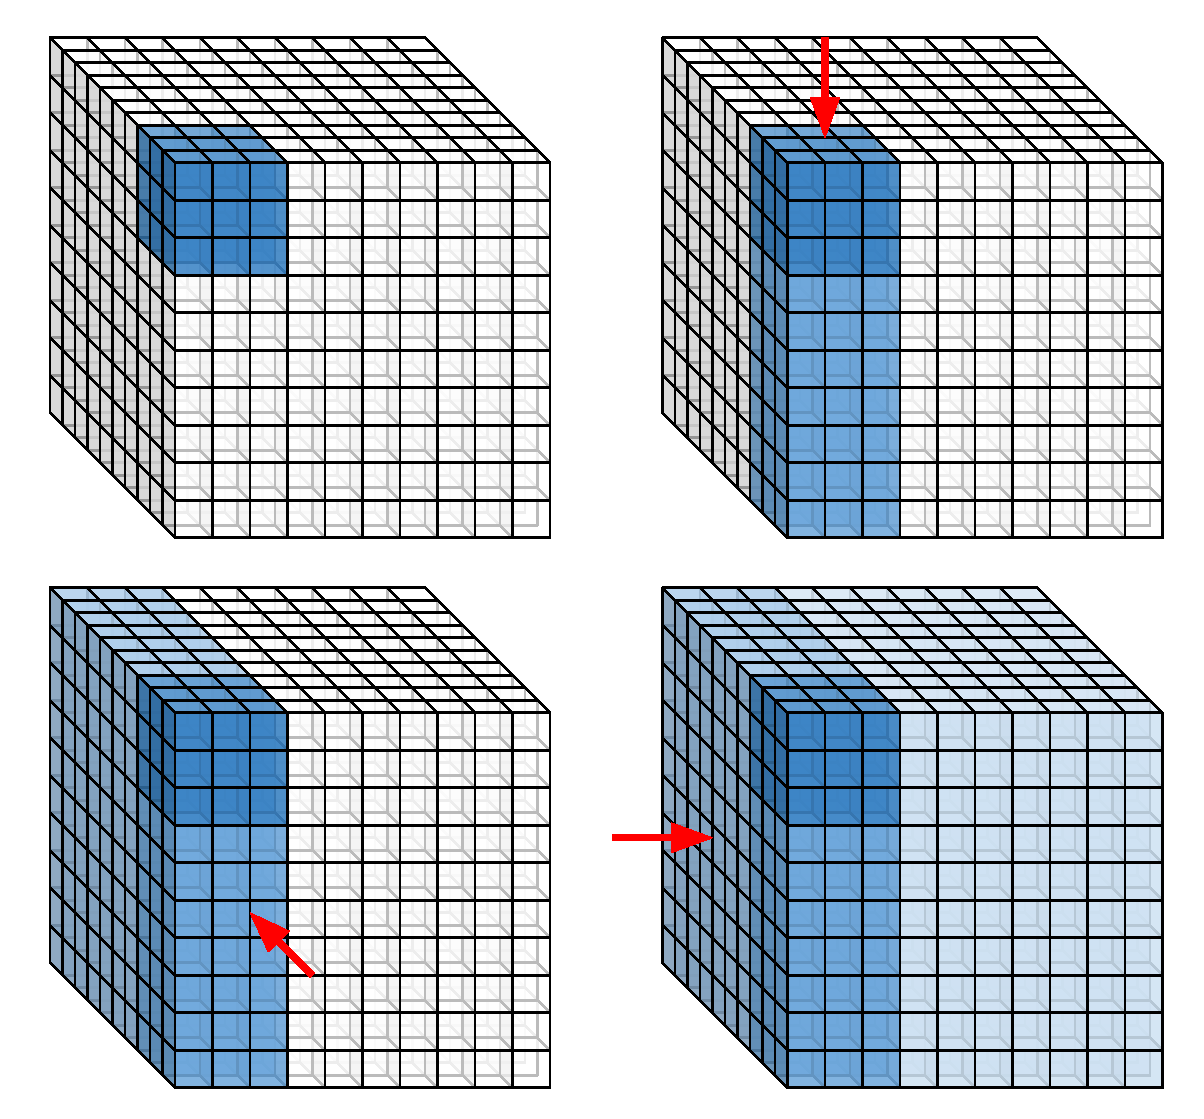
\includegraphics[width=0.8\columnwidth]{fig/pruned_ffts.pdf}
  \end{center}
  \caption{Pruned FFTs.}
  \label{fig:pruned_ffts}
\end{figure}


When computing the FFTs of the trainable kernels we need to zero-pad
the kernels of size $k^3$ to the same size as the image the kernel is
being convolved with ($n^3$).  Naively, we can create a new kernel of
size $n^3$ where only $k^3$ elements are non-zero.  The forward FFT of
the new kernel will take $C n\log n^3$ operations.  As a 3D FFT
transform is computed by performing a series of 1D transforms, many of
the 1D transforms will be performed on arrays with all the elements
equal to $0$.

Pruned FFTs can be computed from the same zero-padded kernel, however
we first perform $k^2$ 1D FFTs along $x$-direction, then $k \cdot n$
1D FFTs along $y$-direction, and finally $n^2$ FFTs along the
$z$-direction.  The total complexity is then reduced from $3C n\log n$
to $C n\log n[k^2 + k \cdot n + n^2]$.

As the value of $k$ will typically be much lower than the value of
$n$, the majority of the 1D FFTs will be performed in the
$z$-direction.  When the image is stored in the row-major order (as it
is in C and C++), most of the 1D FFTs will have the array as a
continuous chunk of memory, thus increasing the cache hits.
Additionally, we can easily store the image in memory such that each
of the 1D arrays in $z$-direction is properly aligned for optimally
leveraging the available SIMD instructions.

On the gpu.  For index calculation we use~\cite{warren2013hacker}

\subsection{GPU implementation}

Assume that we want to compute the FFT transforms of $b$ 3D images
each of size $x_i \times y_i \times z_i$.  We first compute the
optimal size for the transform independently in each of the three
dimensions.  Let it be $x_o \times y_o \times z_o$.  The images are
stored in a row major form in memory as a 4D row major matrix of real
numbers with the dimension of $b \times x_i \times y_i \times z_i$.

We first perform in--place real to complex 1D transforms along the $z$
direction. We prepare the input by extending the 4D matrix along the
$z$ direction to fit the result.  The transform will need to contain
$z_o' = z_o / 2 + 1$ complex numbers, and we need twice as many reals.
A matrix of size $b \times x_i \times y_i \times 2z_o')$ is first
initialized to zero, and appropriate elements from the input are
filled in.  After batched in--place real to complex 1D transforms are
performed the result represents a 4D matrix of complex numbers of size
$b \times x_i \times y_i \times z_o'$.  Note that all the 1D
transforms are done on contiguous memory chunks (along the last
dimension).

In the next step we perform in-place complex to complex transforms
along the $y$ direction.  To do that we will flip the dimensions and
zero pad the previous matrix.  First we initialize a matrix of complex
numbers with the size of $b \times x_i \times z_o' \times y_o$.  The
matrix is first initialized to zero.  Each element $i,j,k,l$ of the
input matrix is mapped to $i,j,l,k$.  Then $b \times x_i \times z_o'$
1D transforms are performed along the last dimension (with all
elements contiguous in memory).

Finally we perform the last in-place complex to complex transform
along the $x$ direction.  For that we initialize $b \times z_o' \times
y_o \times x_o$ matrix to all zeros.  An element $i,j,k,l$ from the
previous result gets mapped to an element $i,k,l,j$.  Once again we
perform $b \times z_o' \times y_o$ 1D in--place transforms, once again
on contiguous chunks.

We keep this as the output shape, as we only care about being able to
perform point--wise operations on the image transform.  The backward
transform is done in a similar fashion just taking the steps in the
reverse.

4D matrix reshaping requires a lot of index to index calculation,
which can involve a lot expensive division and modulus operations.
Sometimes these operations are more expensive than the actual 1D
transforms performed.  We improve the performances by only using
multiplications by a pre--computed magic numbers and shift operations
as described in ~\cite{warren2013hacker}.  Image reshaping is easily
implemented using the Thrust CUDA library~\cite{bell2011thrust}.


\begin{algorithm}
  {\small
  \begin{codebox}
    \Procname{$\proc{Linear-index-map}(i,x_i,y_i,y_o)$}
    \li $b \gets i / y_i$
    \li $i \gets i - b \times y_i$
    \li $r \gets b / x_i$
    \li $b \gets b - r \times x_i$
    \li \Return $(r \times y_i + i) \times y_o + b$
  \end{codebox}
  }

  \caption{Index mapping between two 3D matrices.  The input matrix
  had dimensions $b \times x_i \times y_i$, and the output $b \times
  y_i \times y_o$} \label{alg:index_map}
\end{algorithm}


\section{Serial}

Tables for serial execution.

\begin{table*}
  \centering
  \begin{tabular}{ll}
    \hline
    Method    &FLOPs
    \\ \hline
    Direct & $b \cdot f' \cdot f \cdot n'^3 \cdot k^3$
    \\
    Na\"{\i}ve FFTs & $3Cn^3 \log n[bf'+bf+f' \cdot f] + 4bf' \cdot f \cdot n^3$
    \\
    Memoized FFTs & $3bCn^3 \log n[f'+f] + 4bf' \cdot f \cdot n^3$
    \\
    Pruned FFTs & $3bCn^3 \log n[f'+f] + C n\log n[k^2 + k \cdot n + n^2] \cdot f' \cdot f + 4bf' \cdot f \cdot n^3$
    \\ \hline
  \end{tabular}
  \caption{Computational complexity of a fully connected convolutional
    layer, which maps $f$ input images to $f'$ output images using
    $ff'$ kernels. FFT complexity for an array of $n$ elements is
    assumed to be $Cn\log n$.  Complexity is measured in number of
    floating point operations.}
  \label{table:conv_complexity}
\end{table*}


\begin{table}
  \centering
  \begin{tabular}{llll}
    \hline
    Method    &Images   &Stack   &Memoized
    \\ \hline
    Direct & $f \cdot b \cdot n^3 + f' \cdot b \cdot n'^3$ & - & -
    \\
    Na\"{\i}ve FFTs & $[f + f'] \cdot b \cdot  n^3$ & $2n^3$ & -
    \\
    Memoized FFTs & $[f + f'] \cdot b \cdot  n^3$ & - & $f' \cdot f \cdot n^3$
    \\
    Pruned FFTs & $[f + f'] \cdot b \cdot  n^3$ & $k^2n + n^3$ & -
    \\ \hline
  \end{tabular}
  \caption{Memory usage in number of floating point numbers. $b$ is
    the batch size.}
  \label{table:conv_memory}
\end{table}


\section{Parallel}

Tables for parallel execution.  Explain the parallelization strategies
-- they are different then ZNN training.

ZNN training parallelization strategy:

\begin{itemize}
\item GOOD -- possible better parallelization on large number of cores.
\item BAD -- MUCH more stack memory required -- limits image size
\item BAD -- more instructions (mul to spare memory then add to the sum)
\end{itemize}

Generally, the lock-free summation might not be the best choice here.

\begin{table}
  \centering
  \begin{tabular}{ll}
    \hline
    Method    &FLOPs
    \\ \hline
    Direct & $bf \cdot n'^3 \cdot k^3$
    \\
    Na\"{\i}ve FFTs & $3Cn^3 \log n[2b + f] + 4b f \cdot n^3$
    \\
    Memoized FFTs & $6bCn^3 \log n + 4b f \cdot n^3$
    \\
    Pruned FFTs & $6bCn^3 \log n + C n\log n[k^2 + k \cdot n + n^2] \cdot f + 4b f \cdot n^3$
    \\ \hline
  \end{tabular}
  \caption{Computational complexity of a fully connected convolutional
    layer, which maps $f$ input images to $f'$ output images using
    $ff'$ kernels. FFT complexity for an array of $n$ elements is
    assumed to be $Cn\log n$.  Complexity is measured in number of
    floating point operations.}
  \label{table:conv_complexity}
\end{table}


\begin{table}
  \centering
  \begin{tabular}{llll}
    \hline
    Method    &Images   &Stack   &Memoized
    \\ \hline
    Direct & $f \cdot b \cdot n^3 + f' \cdot b \cdot n'^3$ & - & -
    \\
    Na\"{\i}ve FFTs & $[f + f'] \cdot b \cdot  n^3$ & $T \cdot 2n^3$ & -
    \\
    Memoized FFTs & $[f + f'] \cdot b \cdot  n^3$ & - & $f' \cdot f \cdot n^3$
    \\
    Pruned FFTs & $[f + f'] \cdot b \cdot  n^3$ & $T \cdot [k^2n + n^3]$ & -
    \\ \hline
  \end{tabular}
  \caption{Memory usage in number of floating point numbers. $b$ is
    the batch size.  $T$ is the number of threads.}
  \label{table:conv_memory}
\end{table}

\section{Sliding window inference}

We describe how sliding window works.  Reference ZNN paper and other
papers.  Explain a bit about our implementation.

Also explain how sparse inference works, as we will use that on the
GPU -- only available implementation in 3D.

Explain how the FLOPs per output voxels are computed.

Figures -- chars of FLOPS vs Memory for different algorithms.

Note -- The tables in the previous section are correct even when
rarefied kernels are used, the only thing that changes is the size of
the output image that now equals $n' = n - (k-1)*r$, where $r$ is the
sparseness of the kernel.

\section{CPU Algorithms}

\subsection{Task package and task execution}

We introduce a notion of a task package.  A task package is a set of
independent tasks that we want executed in an arbitrary order, and
which can be executed in parallel.  A task package will be executed by
a thread pool of $N$ running threads.  In order to minimize the
synchronization we do the following two optimization:

All the threads are pre-spawn and are waiting on a condition variable
to start executing the tasks from the task package.

All the tasks in the task package are inserted before the execution
start.  They are inserted onto a lock-free queue from which they will
be picked up by some of the $N$ running threads.

\subsection{Convolutional layers}

The convolutional layers are processed in 3 stages.  In the first
stage, the FFTs of the inputs are computed.  For each input image of
each batch a single task is created.  The tasks are then executed in
parallel.

After the first stage the memory storing the input image can be freed
as the data is not required anymore.

In the second stage the FFTs of the outputs are collected.  A single
task will compute the FFTs of the outputs for a single output image of
each batch.  A network of width $N$ will therefore yield $N$ tasks.
The job if each task is then to compute the FFT of appropriate filters
(one at the time), do a point-wise multiplication and accumulate the
results.

After the second stage the memory where the FFTs of the input images
are stored can be freed.

In the third and final stage we compute the output images.  Each task
here computes an inverse FFT for a single image of a single batch.  A
batch of size $B$ and a network of width $N$ will yield $B \times N$
tasks.  Each task also scales the output appropriately, adds the bias
and applies the transfer function.

\subsection{First layer optimization}

We optimize the first layer to improve the parallelism and reduce the
memory usage.  The problem is that first layer usually has a single
input, and therefore the first stage of the previous algorithm will
utilize only a single core.  Also, the images of the first layer will
be the largest ones, and per-worker requirements for stack memory will
be high.

\section{GPU Algorithms}

Pooling layers use CUDNN.

Direct convolutional layers also use CUDNN.  If possible they use the
precomputed gemm which requires workspace memory.  The cases when this
is possible is not well documented so we experimentally determine
whether we can use it.

FFT convolutional layers are implemented in the following way.  For
each layer we do the following.  We transform all the inputs first.
We break up the input into largest possible chunks that can be
transformed with CUFFTPLANN.  Once we have all the input transforms
(of all the images and bathes) we compute one output image at the
time.  For $i$-th output image we compute FFTs of all the relevant
kernels, then for each batch we compute the point-wise product of the
FFTs of the input images and the FFTs of the kernels.  We accumulate
the result into a single image using a matrix vector product CUBLAS
where the vector has all ones.  We repeat the process for every $i$-th
output of every batch, as we want to re-use the FFTs of the computed
kernels.

Finally we compute the inverse transform of the output images, scale
them appropriately, add the bias and apply the transfer function.

We carefully design the steps in order to minimize the extra memory
utilization.


\section{Experiments}
%%%%%%%%%%%%%%%%%%%%%%%%%%%%%%%%%%%%%%%%%%%%%%%%%%%%%%%%%%%%%%%%%%%%%%%
%%%%%%%%%%%%%%%%%%%%%%%%%%%%%%%%%%%%%%%%%%%%%%%%%%%%%%%%%%%%%%%%%%%%%%%
%%
%% REFERENCES
%%
%%%%%%%%%%%%%%%%%%%%%%%%%%%%%%%%%%%%%%%%%%%%%%%%%%%%%%%%%%%%%%%%%%%%%%%
%%%%%%%%%%%%%%%%%%%%%%%%%%%%%%%%%%%%%%%%%%%%%%%%%%%%%%%%%%%%%%%%%%%%%%%

\IEEEtriggeratref{25}

{\small
\bibliographystyle{IEEEtran}
\bibliography{IEEEabrv,./ref/bib}
}

\end{document}

%% ZNN - A Fast and Furious Technique for Training ConvNets on
%% Multi-Core and Many-Core Shared Memory Machines

%% C = 5 (or 2.5) should be mentioned somewhere?
